\chapter{Experiments and Results}
\label{section:Results}

\todo[inline]{TODO: Update outdated text}
This chapter presents the results accomplished through the execution of the experiments defined in chapter \cref{section:Method}.
First, the results of the ARIMA baselines are presented, containing the tuning of the ARIMA models, as well as the resulting method predictions with these configs.
The second baseline is then pressented, with tuning and testing of the LSTM method.
Lastly, the Convolutional autoencoder and LSTM network is tuned and used on the dataset.


\import{./sections/Results/}{experimental-plan.tex}



\section{Results}
\Cref{table:Average-metric-dataset-1} shows the mean metrics accross
all the time series in dataset 1. The poorest perfoming model accross the board
is SARIMA, with a MASE of $1.294$, sMAPE of $0.239$ and 7 day MASE of $1.063$.
All the different LSTM structures and hybrid methods outperformed SARIMA.

The multivariate models outperformed all the
%% Globale metoder gjør det bedre enn locale på MASE, men dårligere på sMAPE
% Kan det være fordi sMAPE straffer under predictions hardere enn 
% over predictions? TODO: Kjøre eksperiment på nytt for å få figures.

% Globale modeller er dårligere på mase 7 bortsett fra.
% All results tables
\import{./tables/results/dataset_1}{Average-metric-dataset-1.tex}
\import{./tables/results/dataset_2}{Average-metric-dataset-2.tex}
\import{./tables/results/dataset_seasonal}{Average-metric-dataset-seasonal.tex}
\import{./tables/results/dataset_1}{sarima-dataset-1.tex}

\begin{figure}[h!]
  \centering
  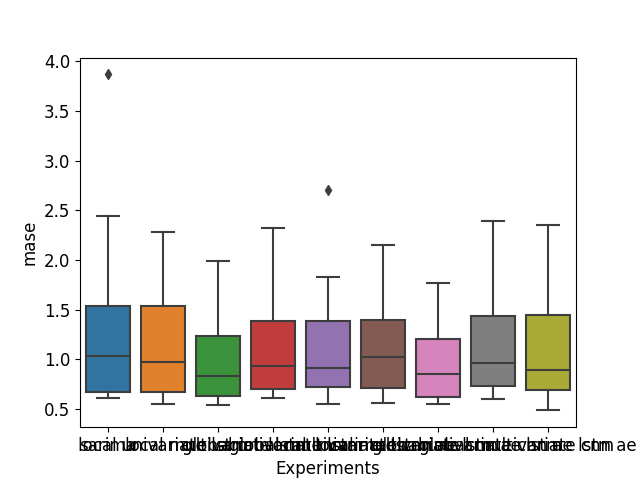
\includegraphics[width=\textwidth]{./figs/results/boxplot/mase-dataset_1.png}
  \hfill
  \caption{TODO..}
  \label{fig:results:boxplot-mase-dataset-1}
\end{figure}

\begin{figure}[h!]
  \centering
  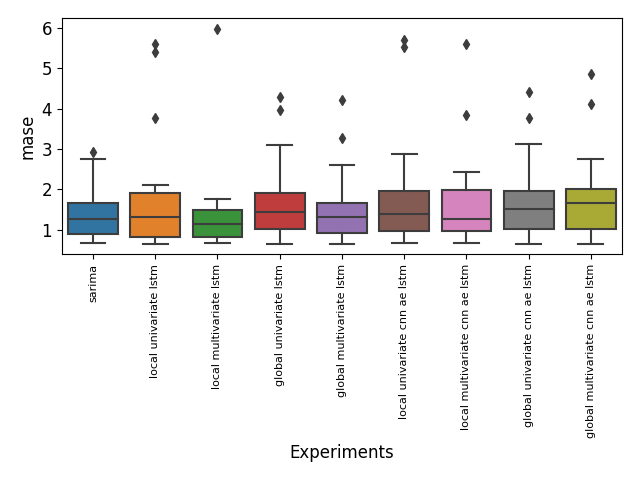
\includegraphics[width=\textwidth]{./figs/results/boxplot/mase-dataset_2.png}
  \hfill
  \caption{TODO..}
  \label{fig:results:boxplot-mase-dataset-2}
\end{figure}



\iffalse

  \section{Experimental Setup}
  \label{sec:experimentalSetup}

  The experimental setup should include all data - parameters etc, that would allow a person to repeat your experiments.

  \section{Experimental Results}
  \label{sec:experimentalResults}

  Results should be clearly displayed and should provide a suitable representation of your results for the points you wish to make. Graphs should be labeled in a legible font and if more than one result is displayed on the same graph then these should be clearly marked.   Please choose carefully rather than presenting every results. Too much information is hard to read and often hides the key information you wish to present. Make use of statistical methods when presenting results, where possible to strengthen the results.  Further, the format of the presentation of results should be chosen based on what issues in the results you wish to highlight. You may wish to present a subset in the experimental section and provide additional results in the appendix.
\fi